\chapter{Bipolar Junction Transistor-Solutions}
\begin{abox}
	Practise Set-1
\end{abox}
\begin{enumerate}
	\item The transistor in the given circuit has $h_{f e}=35 \Omega$ and $h_{i e}=1000 \Omega$. If the load resistance $R_{L}=1000 \Omega$, the voltage and current gain are, respectively.
{	\exyear{NET/JRF(JUNE-2012)}}
\begin{tasks}(1)
	\task[\textbf{A.}] $-35$ and $+35$
	\task[\textbf{B.}] 35 and $-35$
	\task[\textbf{C.}] 35 and $-0.97$
	\task[\textbf{D.}]  $0.98$ and - 35
\end{tasks}
\begin{figure}[H]
	\centering
	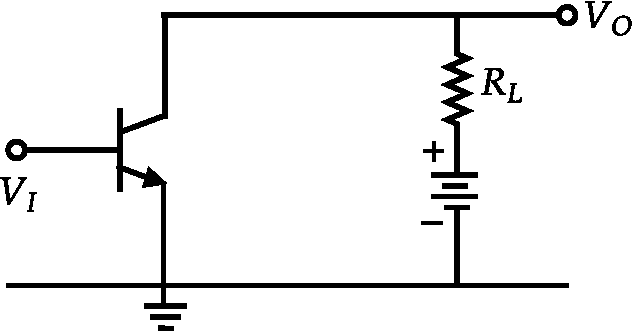
\includegraphics[height=3cm,width=5cm]{e-10}
\end{figure}
\begin{answer}
So the correct answer is \textbf{Option (A)}
\end{answer}
	\item A silicon transistor with built-in voltage $0.7 \mathrm{~V}$ is used in the circuit shown, with $V_{B B}=9.7 V, R_{B}=300 k \Omega, V_{C C}=12 V$ and $R_{C}=2 k \Omega$. Which of the following figures correctly represents the load line and quiescent $Q$ point?
{	\exyear{NET/JRF(JUNE-2013)}}
\begin{figure}[H]
\centering
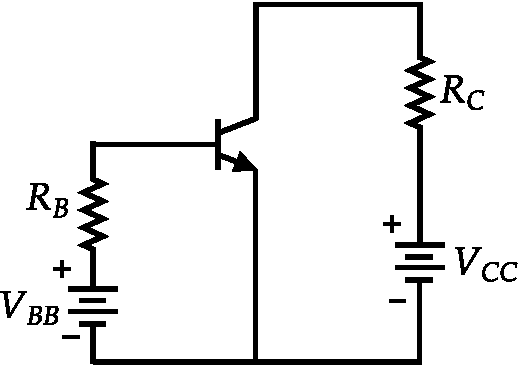
\includegraphics[height=3.5cm,width=5cm]{e-17}
\end{figure}
\begin{tasks}(2)
\task[\textbf{A.}] \begin{figure}[H]
	\centering
	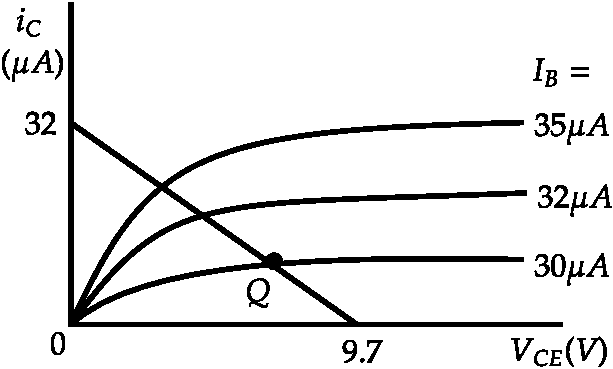
\includegraphics[height=3.3cm,width=5.5cm]{e-17a}
\end{figure}
\task[\textbf{B.}] \begin{figure}[H]
	\centering
	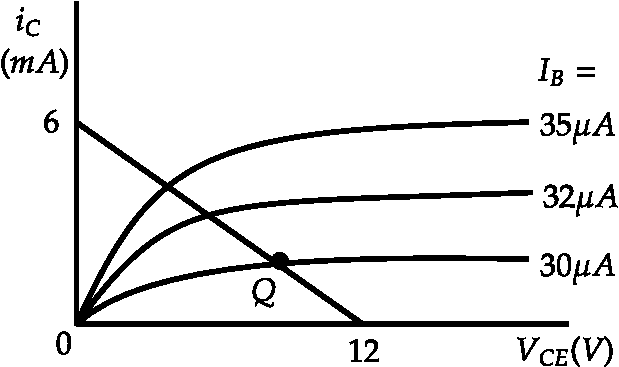
\includegraphics[height=3.3cm,width=5.5cm]{e-17b}
\end{figure}
\task[\textbf{C.}] \begin{figure}[H]
	\centering
	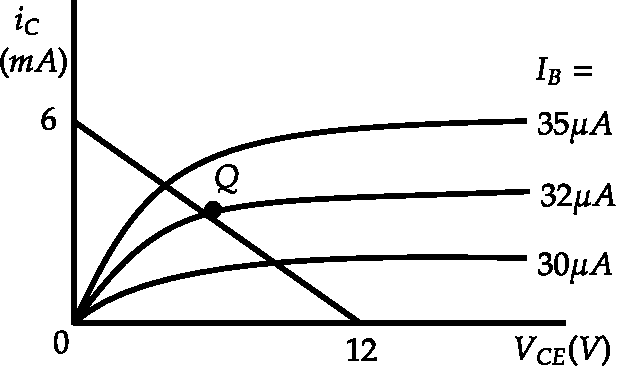
\includegraphics[height=3.3cm,width=5.5cm]{e-17c}
\end{figure}
\task[\textbf{D.}] \begin{figure}[H]
	\centering
	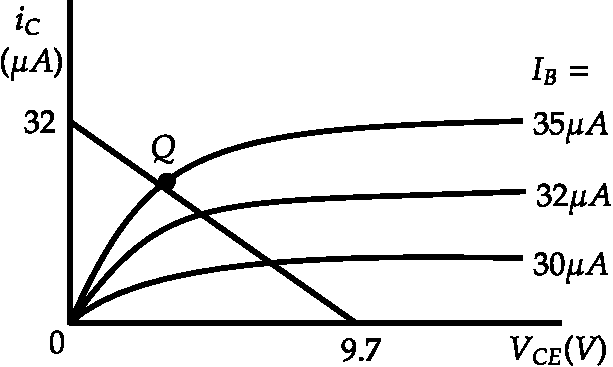
\includegraphics[height=3.3cm,width=5.5cm]{e-17d}
\end{figure}
\end{tasks}
\begin{answer}
\begin{align*}
I_{B}&=\frac{V_{B B}-V_{B E}}{R_{B}}=\frac{9.7-0.7}{300 \times 10^{3}}=30 \mu A\\\text{ and } I_{C, s a t}&=\frac{V_{C C}}{R_{C}}=\frac{12}{2 \times 10^{3}}=6 m A
\end{align*}
So the correct answer is \textbf{Option (B)}
\end{answer}
	\item The input to a lock-in amplifier has the form $V_{i}(t)=V_{i} \sin \left(\omega t+\theta_{i}\right)$ where $V_{i}, \omega, \theta_{i}$ are the amplitude, frequency and phase of the input signal respectively. This signal is multiplied by a reference signal of the same frequency $\omega$, amplitude $V_{r}$ and phase $\theta_{r}$. If the multiplied signal is fed to a low pass filter of cut-off frequency $\omega$, then the final output signal is
{	\exyear{NET/JRF(JUNE-2013)}}
\begin{tasks}(2)
\task[\textbf{A.}] $\frac{1}{2} V_{i} V_{r} \cos \left(\theta_{i}-\theta_{r}\right)$
\task[\textbf{B.}] $V_{i} V_{r}\left[\cos \left(\theta_{i}-\theta_{r}\right)-\cos \left(\frac{1}{2} \omega t+\theta_{i}+\theta_{r}\right)\right]$
\task[\textbf{C.}] $V_{i} V_{r} \sin \left(\theta_{i}-\theta_{r}\right)$
\task[\textbf{D.}] $V_{i} V_{r}\left[\cos \left(\theta_{i}-\theta_{r}\right)+\cos \left(\frac{1}{2} \omega t+\theta_{i}+\theta_{r}\right)\right]$
\end{tasks}
\begin{answer}
\begin{align*}
V&=V_{r} \sin \left(\omega t+\theta_{r}\right) \times V_{i} \sin \left(\omega t+\theta_{i}\right)\\&=\frac{V_{i} V_{r}}{2}\left[\cos \left(\theta_{i}-\theta_{r}\right)-\cos \left(2 \omega t+\theta_{i}+\theta_{r}\right)\right]\\
\text{Output of low pass filter }&=\frac{V_{i} V_{r}}{2} \cos \left(\theta_{i}-\theta_{r}\right)
\end{align*}
So the correct answer is \textbf{Option (A)}
\end{answer}
	\item An $R C$ network produces a phase-shift of $30^{\circ}$. How many such $R C$ networks should be cascaded together and connected to a Common Emitter amplifier so that the final circuit behaves as an oscillator?
{	\exyear{NET/JRF(JUNE-2014)}}
\begin{tasks}(4)
\task[\textbf{A.}] 6
\task[\textbf{B.}] 12
\task[\textbf{C.}] 9
\task[\textbf{D.}] 3
\end{tasks}
\begin{answer}$\left. \right. $\\
Solution: Total phase shift must be 0 or $360^{\circ}$. Common Emitter amplifier has phase change of $180^{\circ}$ so we need $6 R C$ network for next $180^{\circ}$ phase shift.\\
So the correct answer is \textbf{Option (A)}
\end{answer}
	\item Consider the circuits shown in figures (a) and (b) below\\
	\begin{figure}[H]
		\centering
		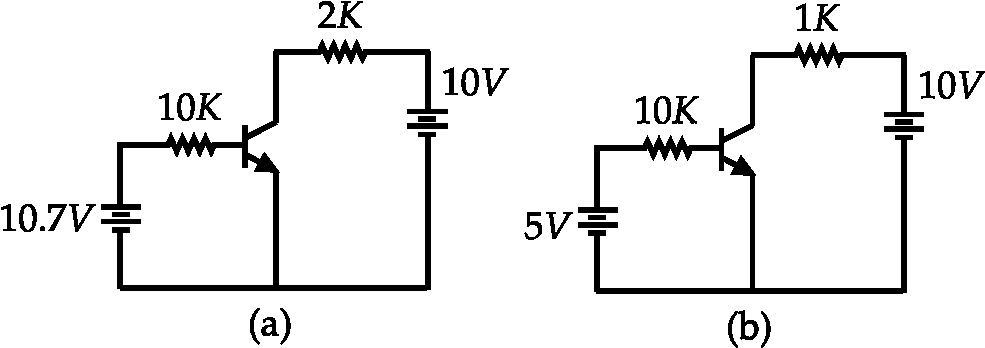
\includegraphics[height=3.2cm,width=9cm]{e-37}
	\end{figure}
	If the transistors in Figures (a) and (b) have current gain $\left(\beta_{d c}\right)$ of 100 and 10 respectively, then they operate in the
{	\exyear{NET/JRF(JUNE-2015)}}
\begin{tasks}(1)
\task[\textbf{A.}] Active region and saturation region respectively
\task[\textbf{B.}] Saturation region and active region respectively
\task[\textbf{C.}] Saturation region in both cases
\task[\textbf{D.}]  Active region in both cases
\end{tasks}
\begin{answer}
\begin{align*}
\intertext{In both case input section is F.B.}
\text{For figure (a) }I_{B}&=\frac{10.7-0.7}{10}=1 \mathrm{~mA} \Rightarrow I_{C}=B I_{B}=100 \mathrm{~mA}\\
\text{Thus }V_{C B}&=V_{C}-V_{B}=(10-2 \times 100)-0.7=-v e\\
&\Rightarrow \quad\text{ output section is F.B.}
\intertext{since both section are F.B. so it is in saturation region.}
\text{For Figure (b) }I_{B}&=\frac{5-0.7}{10}=0.43 \mathrm{~mA} \Rightarrow I_{C}=B I_{B}=4.3 \mathrm{~mA}\\
\text{Thus }V_{C B}&=V_{C}-V_{B}=(10-4.3)-0.7=+v e\\
&\Rightarrow \quad\text{ out put section is R.B.}
\intertext{Thus it is in active region}
\end{align*}
So the correct answer is \textbf{Option (B)}
\end{answer}
	\item The $I-V$ characteristics of a device can be expressed as $I=I_{s}\left[\exp \left(\frac{a V}{T}\right)-1\right]$, where $T$ is the temperature and $a$ and $I_{s}$ are constants independent of $T$ and $V$. Which one of the following plots is correct for a fixed applied voltage $V$ ?
{	\exyear{NET/JRF(DEC-2016)}}
\begin{tasks}(2)
\task[\textbf{A.}] \begin{figure}[H]
	\centering
	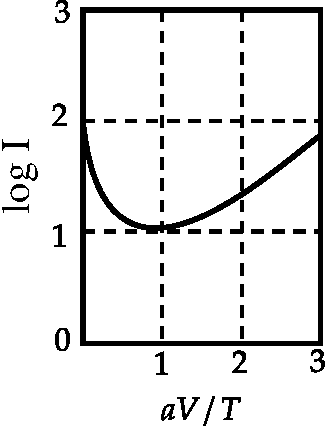
\includegraphics[height=4.5cm,width=3.5cm]{e48a}
\end{figure}
\task[\textbf{B.}] \begin{figure}[H]
	\centering
	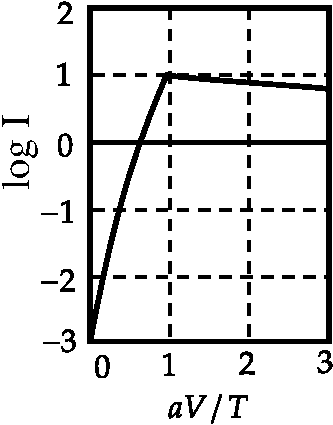
\includegraphics[height=4.5cm,width=3.5cm]{e48b}
\end{figure}
\task[\textbf{C.}] \begin{figure}[H]
	\centering
	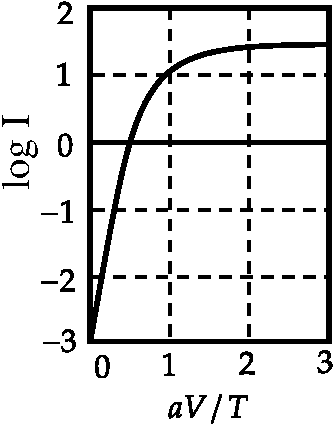
\includegraphics[height=4.5cm,width=3.5cm]{e48c}
\end{figure}
\task[\textbf{D.}] \begin{figure}[H]
	\centering
	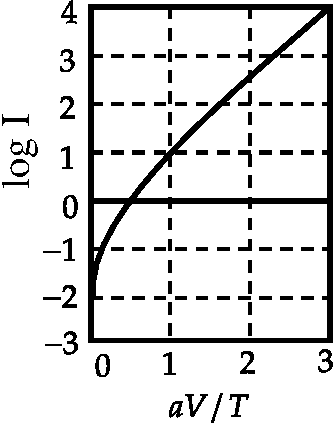
\includegraphics[height=4.5cm,width=3.5cm]{e48d}
\end{figure}
\end{tasks}
\begin{answer}
\begin{align*}
\text{Let }\frac{a v}{T}&=x\text{ For large }x ; \quad I=I_{s} e^{x} \Rightarrow \log _{e} I\\&=\log _{e} I s+x \Rightarrow \log _{e} I \propto x
\end{align*}
So the correct answer is \textbf{Option (D)}
\end{answer}
	\item In the $n$-channel JFET shown in figure below, $V_{i}=-2 V, C=10 p F, V_{D D}=+16 \mathrm{~V}$ and $R_{D}=2 k \Omega$\\
	\begin{figure}[H]
		\centering
		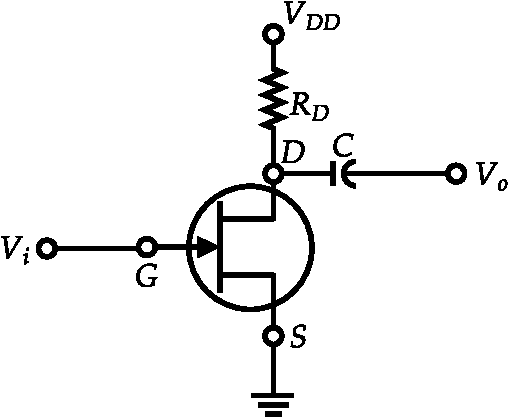
\includegraphics[height=4cm,width=5cm]{e53}
	\end{figure}
	If the drain $D$ - source $S$ saturation current $I_{D S S}$ is $10 m A$ and the pinch-off voltage $V_{P}$ is $-8 V$, then the voltage across points $D$ and $S$ is
{	\exyear{NET/JRF(JUNE-2017)}}
\begin{tasks}(4)
\task[\textbf{A.}] $11.125 \mathrm{~V}$
\task[\textbf{B.}] $10.375 \mathrm{~V}$
\task[\textbf{C.}] $5.75 \mathrm{~V}$
\task[\textbf{D.}] $4.75 \mathrm{~V}$
\end{tasks}
\begin{answer}
\begin{align*}
V_{G S Q}&=-V_{G G}=-2 V\\
I_{D Q}&=I_{D S S}\left(1-\frac{V_{G S}}{V_{P}}\right)^{2}=10 m A\left(1-\frac{-2}{-8}\right)^{2}=5.63 m A\\
V_{D S}&=V_{D D}-I_{D} R_{D}=16-5.63 \times z \approx 4.8 V
\end{align*}
So the correct answer is \textbf{Option (D)}
\end{answer}
	\item In the circuit below the voltages $V_{B B}$ and $V_{C C}$ are kept fixed, the voltage measured at $B$ is a constant, but that measured at $A$ fluctuates between a few $\mu V$ to a few $m V$.\\
	From these measurements it may be inferred that the
	{\exyear{NET/JRF(DEC-2017)}}
\begin{figure}[H]
\centering
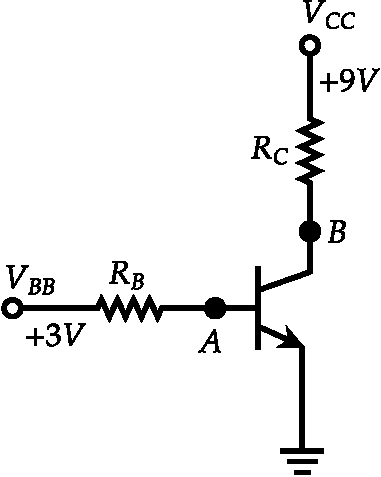
\includegraphics[height=4.5cm,width=4cm]{e63}
\end{figure}
\begin{tasks}(2)
\task[\textbf{A.}] Base is open internally
\task[\textbf{B.}] Emitter is open internally
\task[\textbf{C.}] Collector resistor is open
\task[\textbf{D.}] Base resistor is open
\end{tasks}
\begin{answer}
So the correct answer is \textbf{Option (D)}
\end{answer}
	\item In the following circuit, the value of the common-emitter forward current amplification factor $\beta$ for the transistor is 100 and $V_{B E}$ is $0.7 \mathrm{~V}$.\\
	\begin{figure}[H]
		\centering
		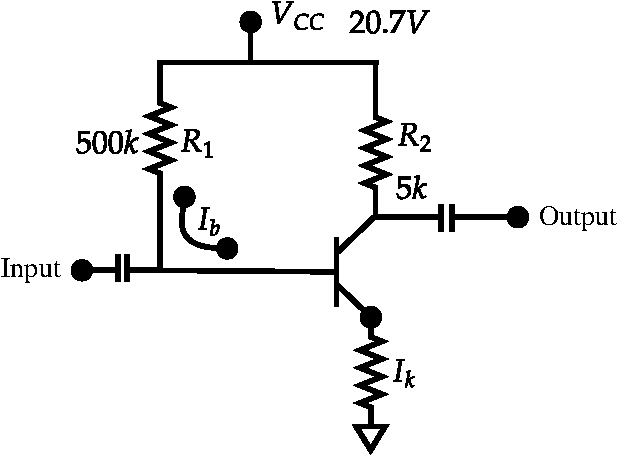
\includegraphics[height=4cm,width=5.5cm]{e68}
	\end{figure}
	The base current $I_{B}$ is
{	\exyear{NET/JRF(JUNE-2018)}}
\begin{tasks}(4)
\task[\textbf{A.}] $40 \mu A$
\task[\textbf{B.}] $30 \mu A$
\task[\textbf{C.}] $44 \mu A$
\task[\textbf{D.}] $33 \mu A$
\end{tasks}
\begin{answer}
\begin{align*}
I_{B}&=\frac{V_{c c}-V_{B E}}{R_{B}+\beta R_{E}}=\frac{20.7-0.7}{500+100 \times 1}\\&=\frac{20}{600 K}=\frac{20 \times 1000}{600} \mu A=33.3 \mu A
\end{align*}
So the correct answer is \textbf{Option (D)}
\end{answer}
	\item A sinusoidal signal is an input to the following circuit\\
	\begin{figure}[H]
		\centering
		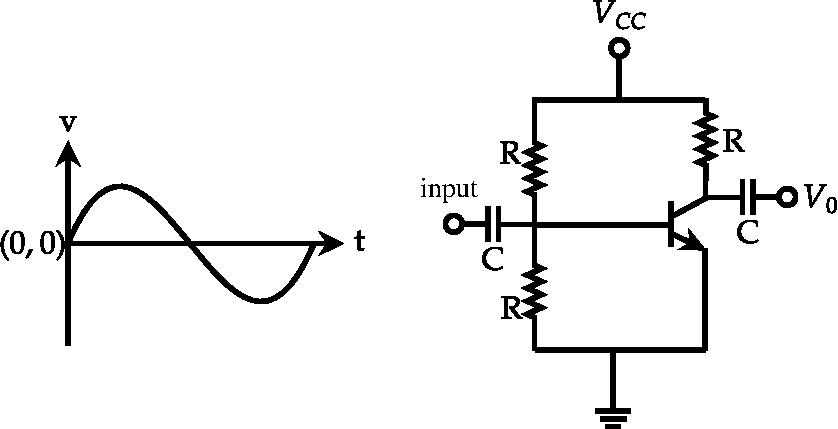
\includegraphics[height=5cm,width=8cm]{e75}
	\end{figure}
	Which of the following graphs best describes the output wave function?
{	\exyear{NET/JRF(DEC-2018)}}
\begin{tasks}(2)
\task[\textbf{A.}] \begin{figure}[H]
	\centering
	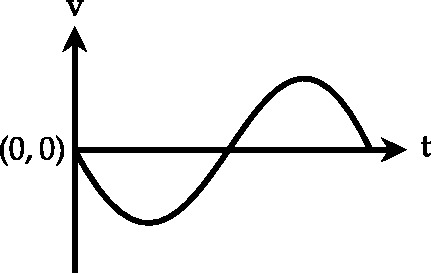
\includegraphics[height=3cm,width=5cm]{e75a}
\end{figure}
\task[\textbf{B.}] \begin{figure}[H]
	\centering
	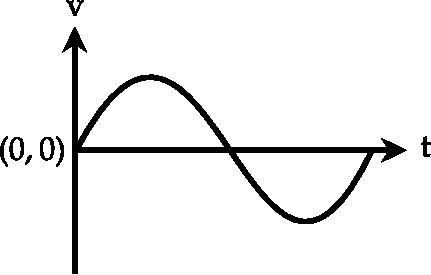
\includegraphics[height=3cm,width=5cm]{e75b}
\end{figure}
\task[\textbf{C.}] \begin{figure}[H]
	\centering
	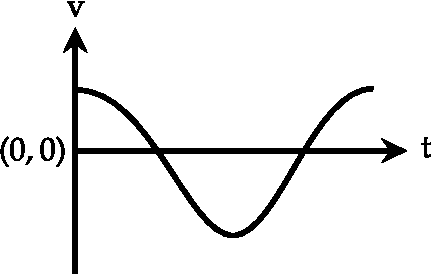
\includegraphics[height=3cm,width=5cm]{e75c}
\end{figure}
\task[\textbf{D.}] \begin{figure}[H]
	\centering
	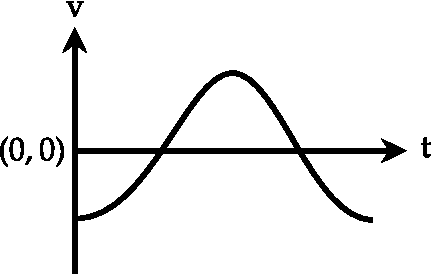
\includegraphics[height=3cm,width=5cm]{e76d}
\end{figure}
\end{tasks}
\begin{answer}
\begin{align*}
\text{In $CE$ transistor output has phase charge of $\pi$}
\end{align*}
So the correct answer is \textbf{Option (A)}
\end{answer}
	\item An $npn$ -transistor is connected in a voltage divider configuration as shown in the figure below\\
	\begin{figure}[H]
		\centering
		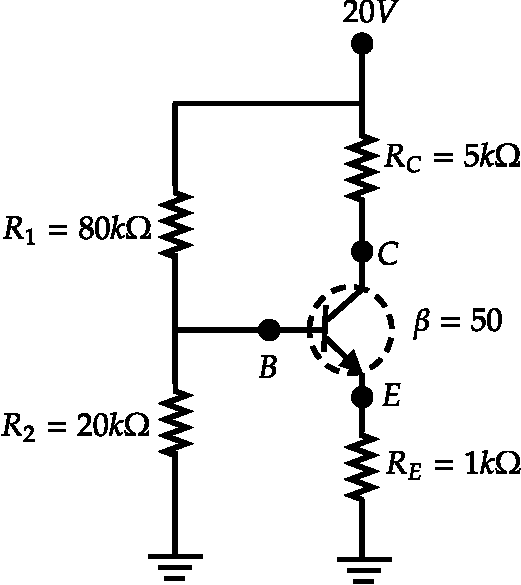
\includegraphics[height=6cm,width=5.5cm]{e-2}
	\end{figure}
	If the resistor $R_{2}$ is disconnected, the voltages $V_{B}$ at the base and $V_{C}$ at the collector change as follows.
{	\exyear{NET/JRF(JUNE-2019)}}
\begin{tasks}(2)
\task[\textbf{A.}]  Both $V_{B}$ and $V_{C}$ increase
\task[\textbf{B.}] Both $V_{B}$ and $V_{C}$ decrease
\task[\textbf{C.}]  $V_{B}$ decreases, but $V_{C}$ increases
\task[\textbf{D.}] $V_{B}$ increases, but $V_{C}$ decreases
\end{tasks}
\begin{answer}
\begin{align*}
V_{B}&=\frac{V_{C C} R_{2}}{R_{1}+R_{2}}=\frac{V_{C C}}{R_{1} / R_{2}+1} \quad\text{ as} R_{2} \uparrow, V_{B} \uparrow\\
\because V_{E}&=V_{B}-V_{B E}\text{ and }I_{E}=\frac{V_{E}}{R_{E}} \approx I_{C}\\
\text{As }&V_{B} \uparrow, V_{E} \uparrow\text{ thus }I_{E} \approx I_{C} \uparrow\\
\because V_{C C}&=V_{C C}-I_{C} R_{c}, \quad\text{ as }I_{C} \uparrow, V_{C} \downarrow
\end{align*}
So the correct answer is \textbf{Option (D)}
\end{answer}
	\item In a collector feedback circuit shown in the figure below, the base emitter voltage $V_{B E}=0.7 V$ and current gain $\beta=\frac{I_{C}}{I_{B}}=100$ for the transistor\\
	\begin{figure}[H]
		\centering
		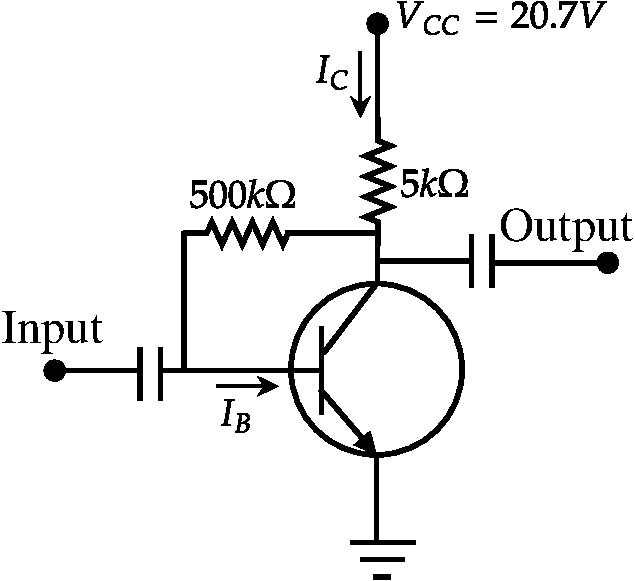
\includegraphics[height=5.5cm,width=6cm]{e-3}
	\end{figure}
	The value of the base current $I_{B}$ is
{	\exyear{NET/JRF(DEC-2019)}}
\begin{tasks}(4)
\task[\textbf{A.}] $20 \mu \mathrm{A}$
\task[\textbf{B.}]  $40 \mu \mathrm{A}$
\task[\textbf{C.}] $10 \mu \mathrm{A}$
\task[\textbf{D.}] $100 \mu \mathrm{A}$
\end{tasks}
\begin{answer}
\begin{align*}
\intertext{Apply K.V.L in input section}
-20 V+B I_{B} \times 5 K+I_{B} \times 500 K+0.7 V&=0\\
\Rightarrow I_{B}=\frac{193}{100 \times 5 K+500 K}&=19.3 \mu \mathrm{A}
\end{align*}
So the correct answer is \textbf{Option (A)}
\end{answer}
\end{enumerate}
\newpage
\begin{abox}
	Practise Set-4
	\end{abox}
\begin{enumerate}
	\item An LED operates at $1.5 \mathrm{~V}$ and $5 \mathrm{~mA}$ in forward bias. Assuming an $80 \%$ external efficiency of the LED, how many photons are emitted per second?
{	\exyear{NET/JRF(JUNE-2012)}}
\begin{tasks}(4)
\task[\textbf{A.}] $5.0 \times 10^{16}$
\task[\textbf{B.}]  $1.5 \times 10^{16}$
\task[\textbf{C.}] $0.8 \times 10^{16}$
\task[\textbf{D.}] $2.5 \times 10^{16}$
\end{tasks}
\begin{answer}
\begin{align*}
P_{i n}&=\eta_{e x t} \frac{i}{e} h f,\text{ number of photon }=\frac{P_{i n}}{h f}\\&=\eta_{e x t} \frac{i}{e}=0.8 \times \frac{5 \times 10^{-3}}{1.6 \times 10^{-19}}=2.5 \times 10^{16}
\end{align*}
So the correct answer is \textbf{Option (D)}
\end{answer}
	\item A sample of $S i$ has electron and hole mobilities of $0.13$ and $0.05 \mathrm{~m}^{2} / \mathrm{V}-\mathrm{s}$ respectively at $300 \mathrm{~K}$. It is doped with $P$ and $A l$ with doping densities of $1.5 \times 10^{21} / \mathrm{m}^{3}$ and $2.5 \times 10^{21} / \mathrm{m}^{3}$ respectively. The conductivity of the doped Si sample at $300 \mathrm{~K}$ is
{	\exyear{NET/JRF(DEC-2013)}}
\begin{tasks}(4)
\task[\textbf{A.}] $8 \Omega^{-1} m^{-1}$
\task[\textbf{B.}] $32 \Omega^{-1} m^{-1}$
\task[\textbf{C.}] $20.8 \Omega^{-1} m^{-1}$
\task[\textbf{D.}] $83.2 \Omega^{-1} m^{-1}$
\end{tasks}
\begin{answer}
\begin{align*}
\intertext{Resulting doped crystal is $p$-type and $p_{p}=(2.5-1.5) \times 10^{21} / \mathrm{m}^{3}=1 \times 10^{21} / \mathrm{m}^{3}$}
\sigma&=e\left(n_{p} \mu_{n}+p_{p} \mu_{p}\right) \approx e p_{p} \mu_{p}\\&=1.6 \times 10^{-19} \times 1 \times 10^{21} \times 0.05=8 \Omega^{-1} m^{-1}
\end{align*}
So the correct answer is \textbf{Option (A)}
\end{answer}
	\item Two identical Zener diodes are placed back to back in series and are connected to a variable DC power supply. The best representation of the $I-V$ characteristics of the circuit is
{	\exyear{NET/JRF(DEC-2013)}}
\begin{tasks}(2)
\task[\textbf{A.}] \begin{figure}[H]
	\centering
	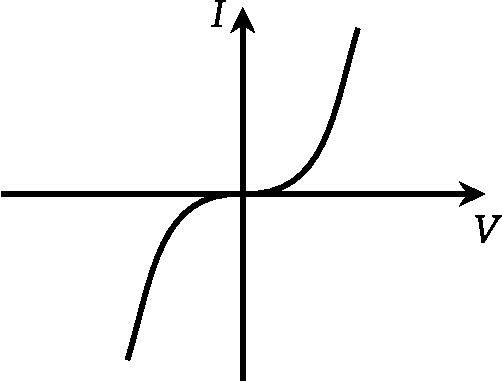
\includegraphics[height=3.5cm,width=4cm]{e-24a}
\end{figure}
\task[\textbf{B.}] \begin{figure}[H]
	\centering
	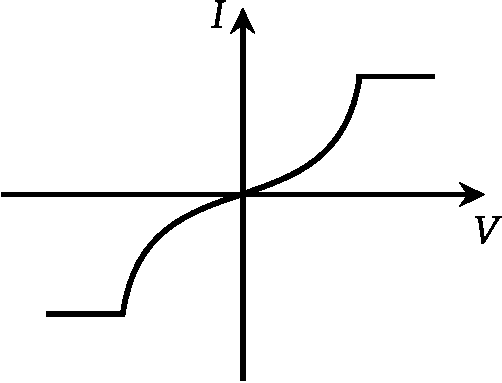
\includegraphics[height=3.5cm,width=4cm]{e-24b}
\end{figure}
\task[\textbf{C.}] \begin{figure}[H]
	\centering
	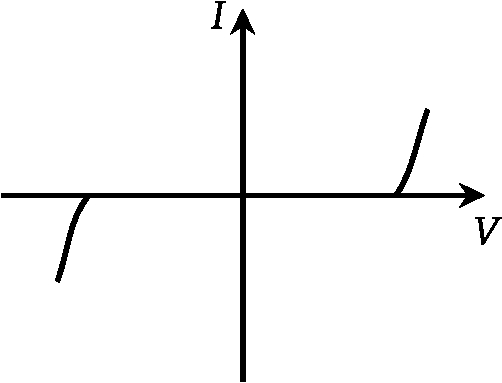
\includegraphics[height=3.5cm,width=4cm]{e-24c}
\end{figure}
\task[\textbf{D.}] \begin{figure}[H]
	\centering
	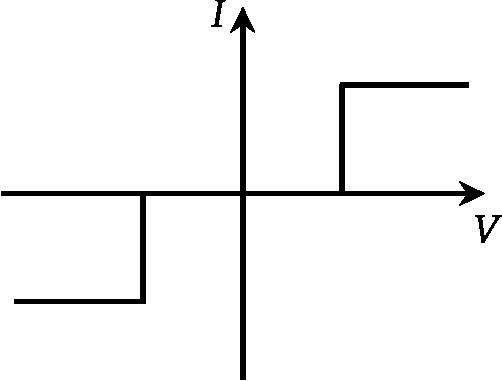
\includegraphics[height=3.5cm,width=4cm]{e-24d}
\end{figure}
\end{tasks}
\begin{answer}
So the correct answer is \textbf{Option (D)}
\end{answer}
	\item The power density of sunlight incident on a solar cell is $100 \mathrm{~mW} / \mathrm{cm}^{2}$. Its short circuit current density is $30 \mathrm{~mA} / \mathrm{cm}^{2}$ and the open circuit voltage is $0.7 \mathrm{~V}$. If the fill factor of the solar cell decreases from $0.8$ to $0.5$ then the percentage efficiency will decrease from
	{\exyear{NET/JRF(DEC-2014)}}
\begin{tasks}(4)
\task[\textbf{A.}] $42.0$ to $26.2$
\task[\textbf{B.}] $24.0$ to $16.8$
\task[\textbf{C.}] $21.0$ to $10.5$
\task[\textbf{D.}] $16.8$ to $10.5$
\end{tasks}
\begin{answer}$\left. \right. $\\
The efficiency of a solar cell is determined as the fraction of incident power which is converted to electricity and is defined as
$$
\eta=\frac{V_{o c} I_{s c} F F}{P_{i n}} \text { and } P_{\max }=V_{o c} I_{s c} F F
$$
where $V_{o c}$ is the open circuit voltage, $I_{s c}$ is the short circuit current density, $F F$ is the Fill factor, $P_{i n}$ is the input power and $\eta$ is the efficiency of the solar cell.
\begin{align*}
\intertext{Given $P_{\text {in }}=100 \mathrm{~mW} / \mathrm{cm}^{2}, I_{s c}=30 \mathrm{~mA} / \mathrm{cm}^{2}, V_{o c}=0.7 \mathrm{~V}$}
\text{	Let $\eta_{1}$ is the efficiency of solar cell when $F$} F&=0.8\\
\therefore \eta_{1}=\frac{(0.7 V) \times\left(30 \times 10^{-3} \mathrm{~A} / \mathrm{cm}^{2}\right) \times 0.8}{100 \times 10^{-3} \mathrm{~W} / \mathrm{cm}^{2}}&=\frac{16.8}{100} \Rightarrow \eta_{1}=0.168\\
\text{Let $\eta_{2}$ is the efficiency of solar cell when $F$ } F=0.5\\
\therefore \eta_{2}=\frac{(0.7 \mathrm{~V}) \times\left(30 \times 10^{-3} \mathrm{~A} / \mathrm{cm}^{2}\right) \times 0.5}{100 \times 10^{-3} \mathrm{~W} / \mathrm{cm}^{2}}&=\frac{10.5}{100} \Rightarrow \eta_{2}=0.105\\
\text{Thus efficiency decreases from }\eta_{1}&=16.8 \%\text{ to }\eta_{2}=10.5 \%
\end{align*}
So the correct answer is \textbf{Option (D)}
\end{answer}
	\item The concentration of electrons, $n$ and holes $p$, for an intrinsic semiconductor at a temperature $T$ can be expressed as $n=p=A T^{\frac{3}{2}} \exp \left(-\frac{E_{g}}{2 k_{B} T}\right)$, where $E_{g}$ is the band gap and $A$ is a constant. If the mobility of both types of carrier is proportional to $T^{\frac{-3}{2}}$, then the log of the conductivity is a linear function of $T^{-1}$, with slope
{	\exyear{NET/JRF(JUNE-2015)}}
\begin{tasks}(4)
\task[\textbf{A.}]$\frac{E_{g}}{\left(2 k_{B}\right)}$
\task[\textbf{B.}] $\frac{E_{g}}{k_{B}}$
\task[\textbf{C.}] $\frac{-E_{g}}{\left(2 k_{B}\right)}$
\task[\textbf{D.}] $\frac{-E_{g}}{k_{B}}$
\end{tasks}
\begin{answer}
\begin{align*}
\sigma_{i}&=n_{i} e\left(\mu_{e}+\mu_{p}\right) \propto T^{\frac{3}{2}} \exp \left(\frac{-E_{g}}{2 k_{B} T}\right) \times T^{\frac{-3}{2}} \Rightarrow \sigma_{i}=C \exp \left(\frac{-E_{g}}{2 k_{B} T}\right)\\
\ln \left(\sigma_{i}\right)&=\frac{E_{g}}{2 k_{B} T}+\ln C \Rightarrow\text{ slope is } \frac{-E_{g}}{2 k_{B}}
\end{align*}
So the correct answer is \textbf{Option (C)}
\end{answer}
	\item The decay constants $f_{p}$ of the heavy pseudo-scalar mesons, in the heavy quark limit, are related to their masses $m_{p}$ by the relation $f_{p}=\frac{a}{\sqrt{m_{p}}}$, where $a$ is an empirical parameter to be determined. The values $m_{p}=(6400 \pm 160) \mathrm{MeV}$ and $f_{p}=(180 \pm 15) \mathrm{MeV}$ correspond to uncorrelated measurements of a meson. The error on the estimate of $a$ is
{	\exyear{NET/JRF(JUNE-2016)}}
\begin{tasks}(4)
\task[\textbf{A.}] $175(\mathrm{MeV})^{\frac{3}{2}}$
\task[\textbf{B.}] $900(\mathrm{MeV})^{\frac{3}{2}}$
\task[\textbf{C.}] $1200(\mathrm{MeV})^{\frac{3}{2}}$
\task[\textbf{D.}] $2400(\mathrm{MeV})^{\frac{3}{2}}$
\end{tasks}
\begin{answer}
\begin{align*}
a&=f_{p} m_{p}^{1 / 2}\\
\sigma_{a}^{2}&=\left(\frac{\partial a}{\partial f_{p}}\right)^{2} \sigma_{f_{p}}^{2}+\left(\frac{\partial a}{\partial m_{p}}\right)^{2} \sigma_{m_{p}}^{2} \Rightarrow \frac{\partial a}{\partial f_{p}}\\&=m_{p}^{1 / 2}\text{ and } \frac{\partial a}{\partial m_{p}}=\frac{f_{p}}{2 m_{p}^{\frac{1}{2}}}\\
\Rightarrow \sigma_{a}^{2}&=m_{p} \sigma_{f_{p}}^{2}+\frac{f_{p}^{2}}{4 m_{p}} \sigma_{m_{p}}^{2} \Rightarrow \frac{\sigma_{a}^{2}}{a^{2}}\\&=\left(\frac{\sigma_{f_{p}}}{f_{p}}\right)^{2}+\left(\frac{\sigma_{m_{p}}}{2 m_{p}}\right)^{2} \Rightarrow \sigma_{a}\\&=a\left[\left(\frac{\sigma_{f_{p}}}{f_{p}}\right)^{2}+\left(\frac{\sigma_{m_{p}}}{2 m_{p}}\right)^{2}\right]^{\frac{1}{2}}	\\
\because a&=f_{p} m_{p}^{1 / 2}=(180 \mathrm{MeV})(6400 \mathrm{MeV})^{1 / 2}\\&=180 \times 80(\mathrm{MeV})^{3 / 2}\\
\left(\frac{\sigma_{f_{p}}}{f_{p}}\right)^{2}&=\left(\frac{15}{180}\right)^{2}=6.9 \times 10^{-3}\text{ and }\left(\frac{\sigma_{m_{p}}}{2 m_{p}}\right)^{2}\\&=\left(\frac{160}{2 \times 6400}\right)^{2}=1.56 \times 10^{-4}\\
\sigma_{a}&=180 \times 80(\mathrm{MeV})^{3 / 2}\left[6.9 \times 10^{-3}+1.56 \times 10^{-4}\right]^{1 / 2}\\&=180 \times 80 \times\left(7 \times 10^{-3}\right)^{1 / 2}(\mathrm{MeV})^{3 / 2}\\
\Rightarrow \sigma_{a}&=1204(\mathrm{MeV})^{3 / 2}
\end{align*}
So the correct answer is \textbf{Option (C)}
\end{answer}
	\item Let $I_{0}$ be the saturation current, $\eta$ the ideality factor and $v_{F}$ and $v_{R}$ the forward and reverse potentials respectively, for a diode. The ratio $R_{R} / R_{F}$ of its reverse and forward resistances $R_{R}$ and $R_{F}$, respectively, varies as (In the following $k_{B}$ is the Boltzmann constant, $T$ is the absolute temperature and $q$ is the charge.)
	{\exyear{NET/JRF(JUNE-2017)}}
\begin{tasks}(2)
\task[\textbf{A.}] $\frac{v_{R}}{v_{F}} \exp \left(\frac{q v_{F}}{\eta k_{B} T}\right)$
\task[\textbf{B.}] $\frac{v_{F}}{v_{R}} \exp \left(\frac{q v_{F}}{\eta k_{B} T}\right)$
\task[\textbf{C.}]  $\frac{v_{R}}{v_{F}} \exp \left(-\frac{q v_{F}}{\eta k_{B} T}\right)$
\task[\textbf{D.}]  $\frac{v_{F}}{v_{R}} \exp \left(-\frac{q v_{F}}{\eta k_{B} T}\right)$
\end{tasks}
\begin{answer}
\begin{align*}
I&=I_{0}\left(e^{V / \eta V_{T}}-1\right), V_{T}=\frac{K T}{q}\\
\frac{R_{R}}{R_{F}}&=\frac{V_{R} / I_{R}}{V_{F} / I_{F}}=\frac{V_{R}}{V_{F}} \times \frac{I_{F}}{I_{R}}\\
\Rightarrow \frac{R_{R}}{R_{F}}&=\frac{V_{R}}{V_{F}} \frac{I_{0} e^{V_{F} / \eta V_{T}}}{I_{0}}=\frac{V_{R}}{V_{F}} \exp \left[\frac{q V_{F}}{\eta K_{T}}\right]
\end{align*}
So the correct answer is \textbf{Option (A)}
\end{answer}
	\item Both the data points and a linear fit to the current vs voltage of a resistor are shown in the graph below.\\
	\begin{figure}[H]
		\centering
		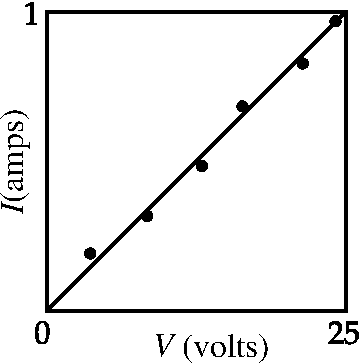
\includegraphics[height=4cm,width=4cm]{e59}
	\end{figure}
	If the error in the slope is $1.255 \times 10^{-3} \Omega^{-1}$, then the value of resistance estimated from the graph is
	{\exyear{NET/JRF(JUNE-2017)}}
\begin{tasks}(4)
\task[\textbf{A.}] $(0.04 \pm 0.8) \Omega$
\task[\textbf{B.}] $(25.0 \pm 0.8) \Omega$
\task[\textbf{C.}] $(25 \pm 1.25) \Omega$
\task[\textbf{D.}] $(25 \pm 0.0125) \Omega$
\end{tasks}
\begin{answer}
\begin{align*}
\text{Slope }&=\frac{I_{\max }-I_{\min }}{V_{\max }-V_{\min }}=\frac{1-0}{25-0}\\&=\frac{1}{25}=m\text{ (let)}\\
\because I&=\frac{V}{R}=m V \Rightarrow R=\frac{1}{m}\\&=25 \Omega\text{ where }\frac{\partial R}{\partial m}=-\frac{1}{m^{2}}\\
\text{Error in $R$ is }\sigma_{R}^{2}&=\left(\frac{\partial R}{\partial m}\right)^{2} \sigma_{m}^{2}=\frac{1}{m^{4}} \sigma_{m}^{2}=R^{4} \sigma_{m}^{2}\\
\Rightarrow \sigma_{R}&=R^{2} \sigma_{m}=(25)^{2} \times 1.255 \times 10^{-3} \approx 0.8 \Omega \\\Rightarrow R&=(25.0 \pm 0.8) \Omega
\end{align*}
So the correct answer is \textbf{Option (B)}
\end{answer}
\item A sinusoidal signal with a peak voltage $V_{p}$ and average value zero, is an input to the following circuit.\\
\begin{figure}[H]
	\centering
	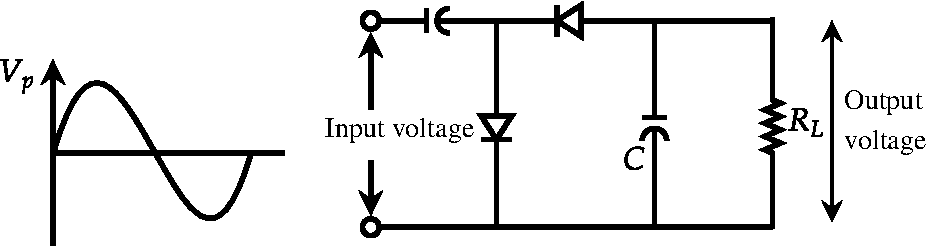
\includegraphics[height=2.5cm,width=9cm]{e67}
\end{figure}
Assuming ideal diodes, the peak value of the output voltage across the load resistor $R_{L}$ is
{\exyear{NET/JRF(JUNE-2018)}}
\begin{tasks}(4)
\task[\textbf{A.}] $V_{p}$
\task[\textbf{B.}] $\frac{V_{p}}{2}$
\task[\textbf{C.}]  $2 V_{p}$
\task[\textbf{D.}]  $\sqrt{2} V_{p}$
\end{tasks}
\begin{answer}
\begin{align*}
\text{It's a voltage doubler circuit}\\
\text{	Peak value }&=2 V_{p}
\end{align*}
So the correct answer is \textbf{Option (C)}
\end{answer}
\item A sinusoidal voltage having a peak value of $V_ p$ is an input to the following circuit, in which the $DC$ voltage is $V_b$ \\
\begin{figure}[H]
	\centering
	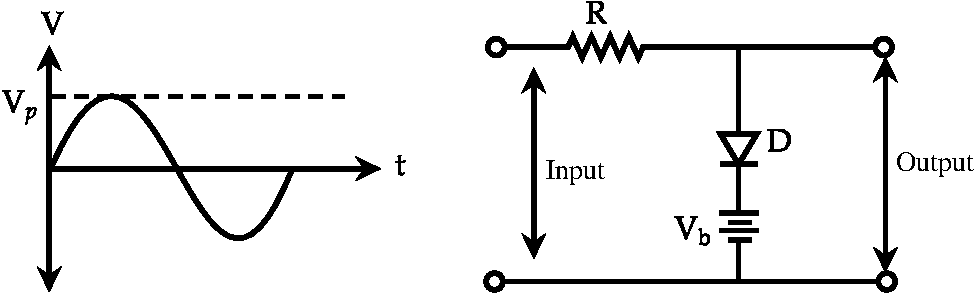
\includegraphics[height=3cm,width=9cm]{e77}
\end{figure}
Assuming an ideal diode which of the following best describes the output waveform?
{\exyear{NET/JRF(DEC-2018)}}
\begin{tasks}(2)
\task[\textbf{A.}] \begin{figure}[H]
	\centering
	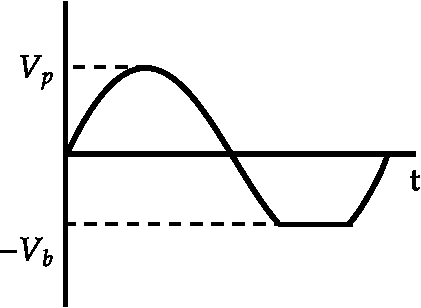
\includegraphics[height=3cm,width=5cm]{e77a}
\end{figure}
\task[\textbf{B.}] \begin{figure}[H]
	\centering
	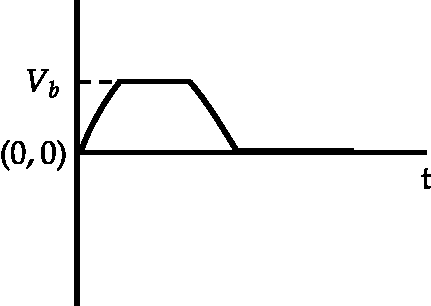
\includegraphics[height=3cm,width=5cm]{e77b}
\end{figure}
\task[\textbf{C.}] \begin{figure}[H]
	\centering
	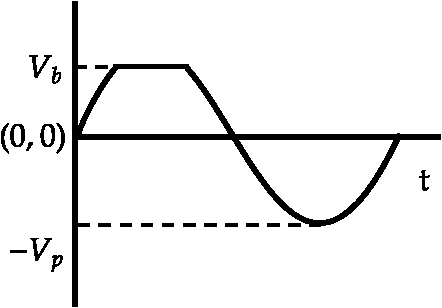
\includegraphics[height=3cm,width=5cm]{e77c}
\end{figure}
\task[\textbf{D.}] \begin{figure}[H]
	\centering
	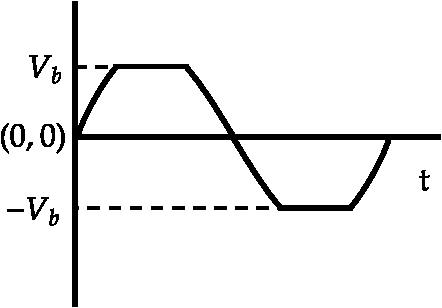
\includegraphics[height=3cm,width=5cm]{e77d}
\end{figure}
\end{tasks}
\begin{answer}
So the correct answer is \textbf{Option (C)}
\end{answer}
\item A $10 V$ battery is connected in series to a resistor $R$ and a capacitor $C$, as shown the figure.\\\begin{figure}[H]
	\centering
	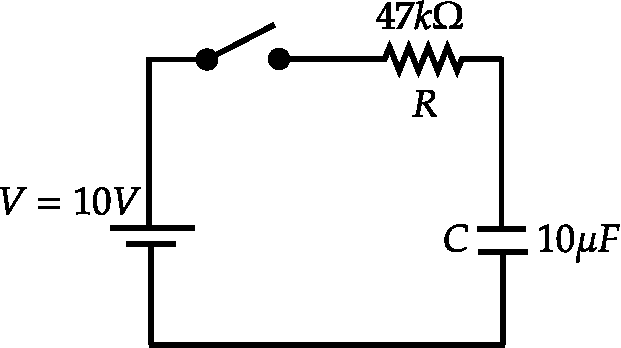
\includegraphics[height=3cm,width=6cm]{BJT-1}
\end{figure}
The initial charge on the capacitor is zero. The switch is turned on and the capacitor is allowed to charge to its full capacity. The total work done by the battery in this process is
{\exyear{NET/JRF(JUNE-2020)}}
\begin{tasks}(4)
\task[\textbf{A.}] $10^{-3} \mathrm{~J}$
\task[\textbf{B.}] $2 \times 10^{-3} \mathrm{~J}$
\task[\textbf{C.}] $5 \times 10^{-4} \mathrm{~J}$
\task[\textbf{D.}] $47 \times 10^{-2} \mathrm{~J}$
\end{tasks}
\begin{answer}
\begin{align*}
\intertext{The total work done by the battery in this process is}
W&=q V=(C V) V=C V^{2}\\&=10 \times 10^{-6} \times(10)^{2}=10^{-3}\text{ Joules}
\end{align*}
So the correct answer is \textbf{Option (A)}
\end{answer}
\item The temperature variation of the resistivity of four materials are shown in the following graphs.
\begin{tasks}(2)
	\task[\textbf{A.}] \begin{figure}[H]
		\centering
		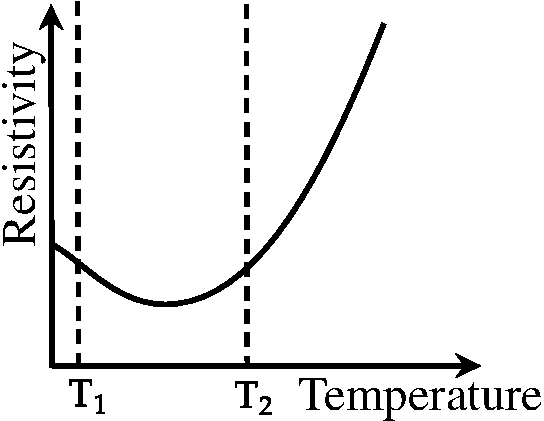
\includegraphics[height=4cm,width=5cm]{BJT-02}
	\end{figure}
	\task[\textbf{B.}]\begin{figure}[H]
		\centering
		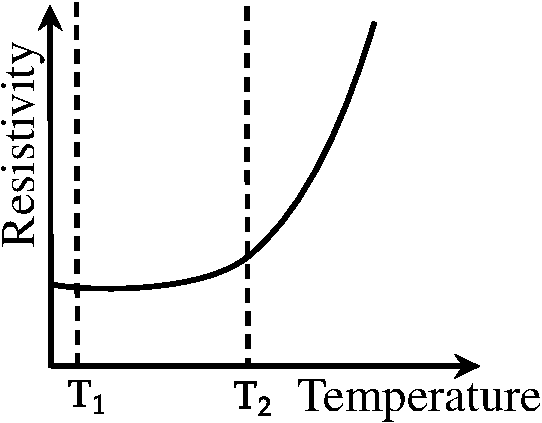
\includegraphics[height=4cm,width=5cm]{BJT-03}
	\end{figure}
	\task[\textbf{C.}] \begin{figure}[H]
		\centering
		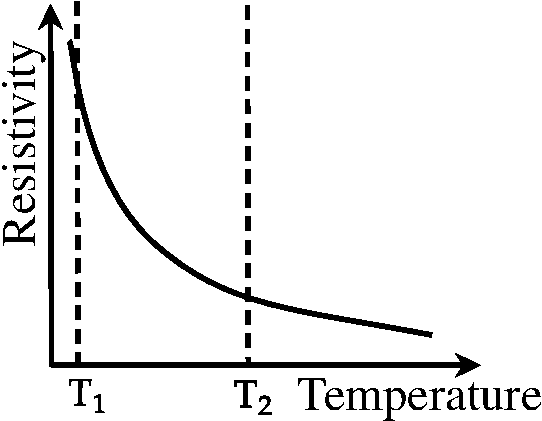
\includegraphics[height=4cm,width=5cm]{BJT-04}
	\end{figure}
	\task[\textbf{D.}] \begin{figure}[H]
		\centering
		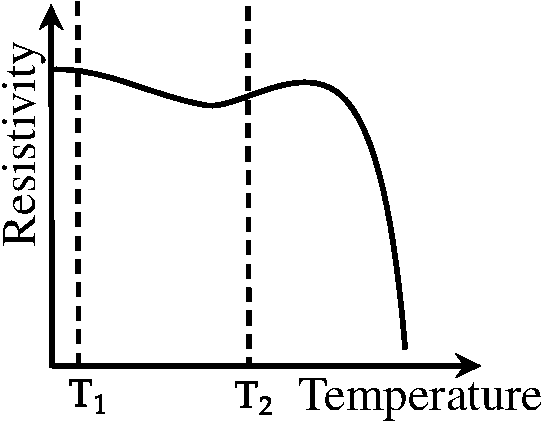
\includegraphics[height=4cm,width=5cm]{BJT-06}
	\end{figure}
\end{tasks}
The material that would make the most sensitive temperature sensor, when used at temperatures between $T_{1}$ and $T_{2}$, is
{\exyear{NET/JRF(JUNE-2020)}}
\begin{tasks}(4)
\task[\textbf{A.}] A
\task[\textbf{B.}] B
\task[\textbf{C.}] C
\task[\textbf{D.}] D
\end{tasks}
\begin{answer}
\begin{align*}
\intertext{ For the temperature sensor, the variation in the resistivity of material should be as large as possible without any local maximum or minimum. Option (A) \& (D) shows minimum while in (B) gradient is very low in comparison to (C). Thus option (C) is the correct answer}
\end{align*}
So the correct answer is \textbf{Option (C)}
\end{answer}
\item Two voltmeters $A$ and $B$ with internal resistances $2 M \Omega$ and $0.1 k \Omega$ are used to measure the voltage drops $V_{A}$ and $V_{B}$, respectively, across the resistor $R$ in the circuit shown below.\\
\begin{figure}[H]
	\centering
	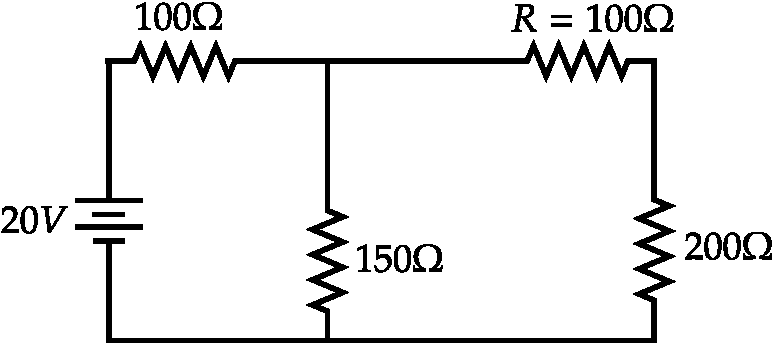
\includegraphics[height=3cm,width=7cm]{BJT-07}
\end{figure}
The ratio $V_{A} / V_{B}$ is
{\exyear{NET/JRF(JUNE-2020)}}
\begin{tasks}(4)
\task[\textbf{A.}] $0.58$
\task[\textbf{B.}] $1.73$
\task[\textbf{C.}] 1
\task[\textbf{D.}] 2
\end{tasks}
\begin{answer}
Let us draw Thevenin’s equivalent across point ab:\\
\begin{figure}[H]
	\centering
	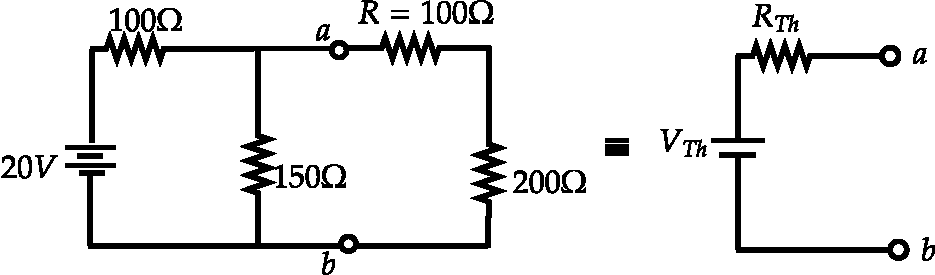
\includegraphics[height=3cm,width=10cm]{BJT-08}
\end{figure}
\begin{figure}[H]
	\centering
	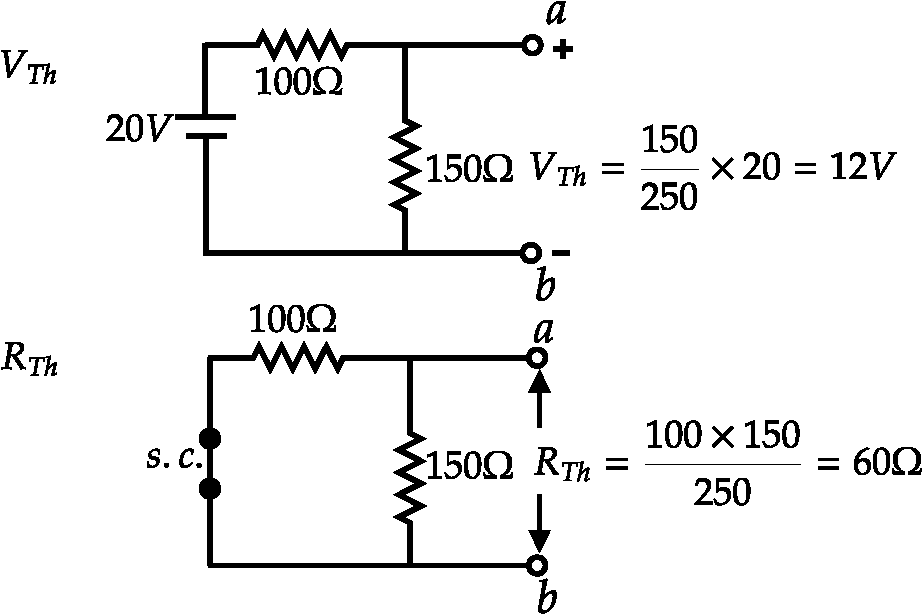
\includegraphics[height=5cm,width=9cm]{BJT-09}
\end{figure}
\textbf{Equivalent circuit:}\\
\begin{figure}[H]
	\centering
	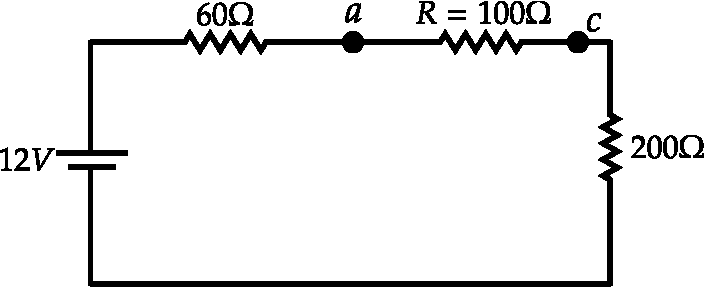
\includegraphics[height=3cm,width=7cm]{BJT-10}
\end{figure}
Voltmeter is connected across point ac in parallel.
\begin{align*}
\intertext{\textbf{Case A:} Voltmeter internal resistance is $2M\Omega $ , so equivalent resistance across ac is}
&=\frac{100 \Omega \times 2 M \Omega}{100 \Omega+2 M \Omega} \approx 100 \Omega\\
\text{So }V_{A}&=\frac{100}{360} \times 12 V=\frac{10}{3} V
\intertext{\textbf{Case B:} Voltmeter internal resistance is $0.1 \mathrm{k} \Omega=100 \Omega$, so equivalent resistance across ac is}
&=\frac{100 \Omega \times 100 \Omega}{100 \Omega+100 \Omega}=50 \Omega\\
\text{So }V_{B}&=\frac{50}{310} \times 12 V=\frac{600}{310} V=\frac{60}{31} V\\
\Rightarrow \frac{V_{A}}{V_{B}}&=\frac{10 / 3}{60 / 31}=\frac{10}{60} \times \frac{31}{3}=1.72
\end{align*}
So the correct answer is \textbf{Option (B)}
\end{answer}
\item The $I-V$ characteristics of the diode $D$ in the circuit below is given by
$$
I=I_{s}\left(e^{\frac{q V}{k_{\mathrm{B}} T}}-1\right)
$$
where $I_{s}$ is the reverse saturation current, $V$ is the voltage across the diode and $T$ is the absolute temperature.\\
\begin{figure}[H]
	\centering
	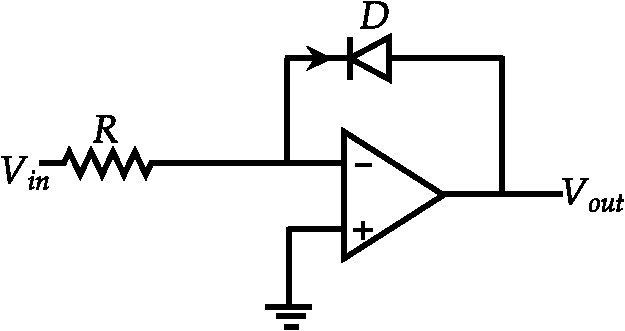
\includegraphics[height=3.5cm,width=6cm]{BJT-11}
\end{figure}
If the input voltage is $V_{\text {in }}$, then the output voltage $V_{\text {out }}$ is
{\exyear{NET/JRF(JUNE-2020)}}
\begin{tasks}(2)
\task[\textbf{A.}] (a) $I_{s} R \ln \left(\frac{q V_{\text {in }}}{k_{B} T}+1\right)$
\task[\textbf{B.}] $\frac{1}{q} k_{B} T \ln \left(\frac{q\left(V_{\text {in }}+I_{s} R\right)}{k_{B} T}\right)$
\task[\textbf{C.}]  $\frac{1}{q} k_{B} T \ln \left(\frac{V_{\text {in }}}{I_{s} R}+1\right)$
\task[\textbf{D.}]  $-\frac{1}{q} k_{B} T \ln \left(\frac{V_{\text {in }}}{I_{s} R}+1\right)$
\end{tasks}
\begin{answer}
\begin{align*}
\because I&=I_{R} \quad \Rightarrow I_{S}\left(e^{e V_{D} / k_{B} T}-1\right)=\frac{0-\left(-V_{i n}\right)}{R}\\
\\\Rightarrow e^{e V_{D} / k_{B} T}-1&=+\frac{V_{i n}}{I_{S} R} \Rightarrow e^{e V_{D} / k_{B} T}\\&=\frac{V_{i n}}{I_{S} R}+1 \Rightarrow V_{D}=\frac{k_{B} T}{e} \ln \left(\frac{V_{\text {in }}}{I_{S} R}+1\right)
\end{align*}
So the correct answer is \textbf{Option (C)}
\end{answer}
\end{enumerate}
\newpage
\begin{abox}
	Practise set-2
	\end{abox}
\begin{enumerate}
	\item Which of the following statements is CORRECT for a common emitter amplifier circuit?
{	\exyear{GATE 2011}}
\begin{tasks}(1)
\task[\textbf{A.}] The output is taken from the emitter
\task[\textbf{B.}] There is $180^{\circ}$ phase shift between input and output voltages
\task[\textbf{C.}] There is no phase shift between input and output voltages
\task[\textbf{D.}] Both $p-n$ junctions are forward biased
\end{tasks}
\begin{answer}
So the correct answer is \textbf{Option (B)}
\end{answer}
\item 	In the following circuit, Trl and $\operatorname{Tr} 2$ are identical transistors having $V_{B E}=0.7 \mathrm{~V}$. The current passing through the transistor $\operatorname{Tr} 2$ is
{\exyear{GATE 2011}}
\begin{figure}[H]
\centering
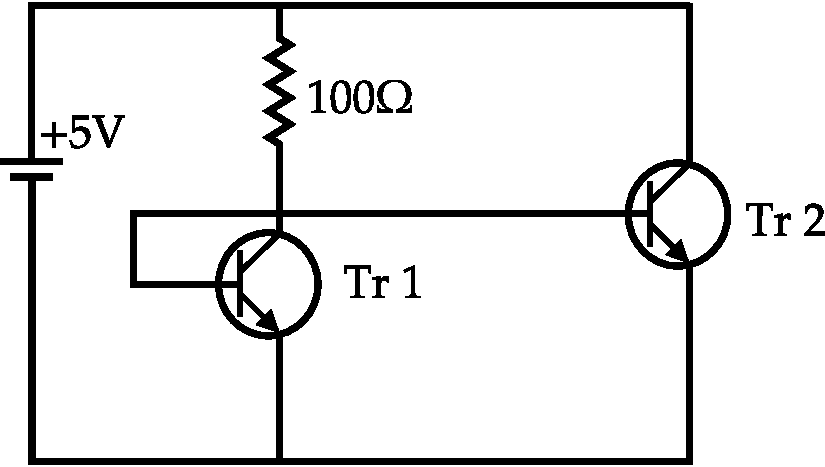
\includegraphics[height=4.5cm,width=8cm]{BJT-40}
\end{figure}
\begin{tasks}(4)
\task[\textbf{A.}] $57 \mathrm{~mA}$
\task[\textbf{B.}] $50 \mathrm{~mA}$
\task[\textbf{C.}] $48 \mathrm{~mA}$
\task[\textbf{D.}] $43 \mathrm{~mA}$
\end{tasks}
\begin{answer}
\begin{align*}
\text{	Current through }100 \Omega, I&=\frac{5-0.7}{100}=43 \mathrm{~mA}\\
I&=I_{C}+2 I_{B} \approx I_{C}=43 \mathrm{~mA}
\end{align*}
So the correct answer is \textbf{Option (D)}
\end{answer}
	\item If the peak output voltage of a full wave rectifier is $10 \mathrm{~V}$, its d.c. voltage is
{	\exyear{GATE 2012}}
\begin{tasks}(4)
\task[\textbf{A.}] $10.0 \mathrm{~V}$
\task[\textbf{B.}] $7.07 \mathrm{~V}$
\task[\textbf{C.}] $6.36 \mathrm{~V}$
\task[\textbf{D.}] $3.18 \mathrm{~V}$
\end{tasks}
\begin{answer}
\begin{align*}
V_{d c}&=\frac{2 V_{m}}{\pi}=\frac{2 \times 10}{22 / 7}\\&=\frac{14 \times 10}{22}=\frac{70}{11}=6.36 \mathrm{~V}
\end{align*}
So the correct answer is \textbf{Option (C)}
\end{answer}
	\item Consider the following circuit in which the current gain $\beta_{d c}$ of the transistor is 100 .\\
	\begin{figure}[H]
		\centering
		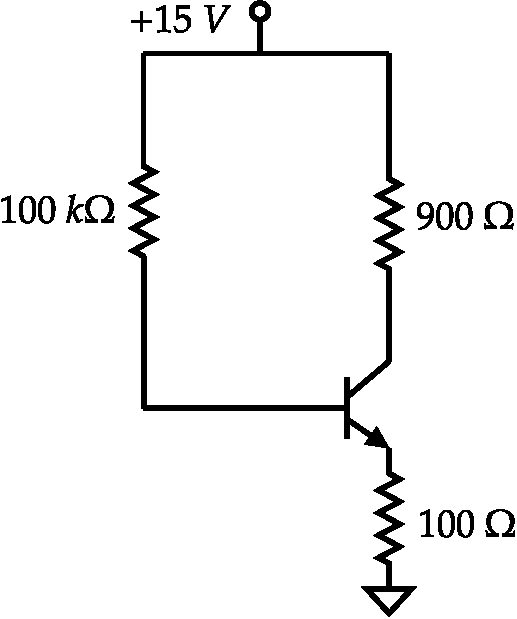
\includegraphics[height=6cm,width=5cm]{BJT-41}
	\end{figure}
	Which one of the following correctly represents the load line (collector current $\mathrm{I}_{\mathrm{C}}$ with respect to collector-emitter voltage $\mathrm{V}_{\mathrm{CE}}$ ) and Q-point of this circuit?
{	\exyear{GATE 2012}}
\begin{tasks}(2)
\task[\textbf{A.}]\begin{figure}[H]
	\centering
	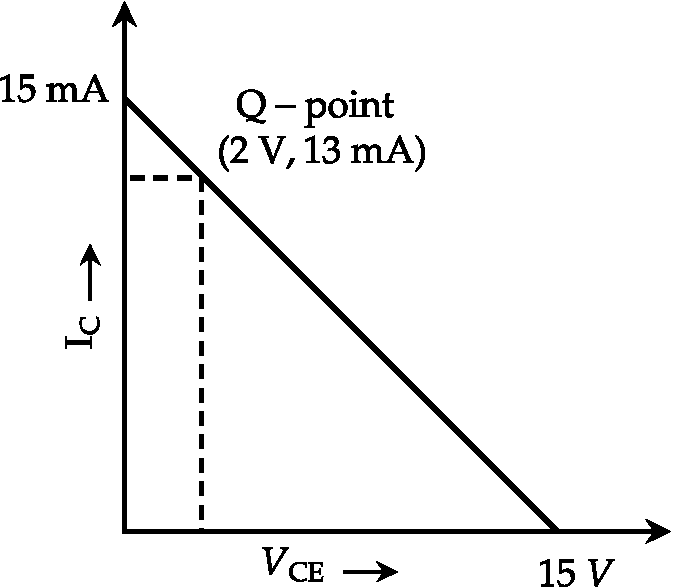
\includegraphics[height=4.5cm,width=5cm]{BJT-42}
\end{figure}
\task[\textbf{B.}] \begin{figure}[H]
	\centering
	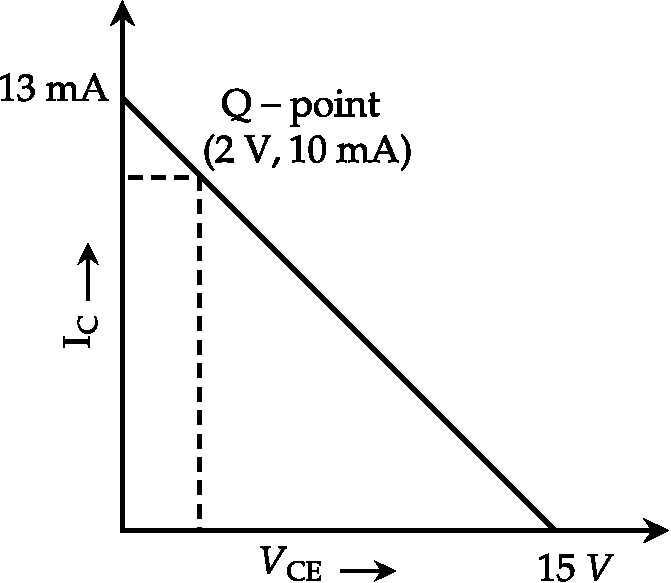
\includegraphics[height=4.5cm,width=5cm]{BJT-43}
\end{figure}
\task[\textbf{C.}] \begin{figure}[H]
	\centering
	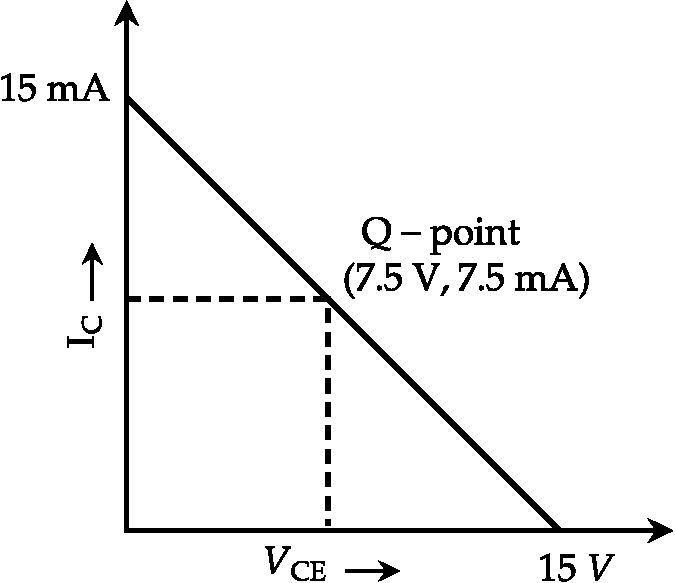
\includegraphics[height=4.5cm,width=5cm]{BJT-44}
\end{figure}
\task[\textbf{D.}] \begin{figure}[H]
	\centering
	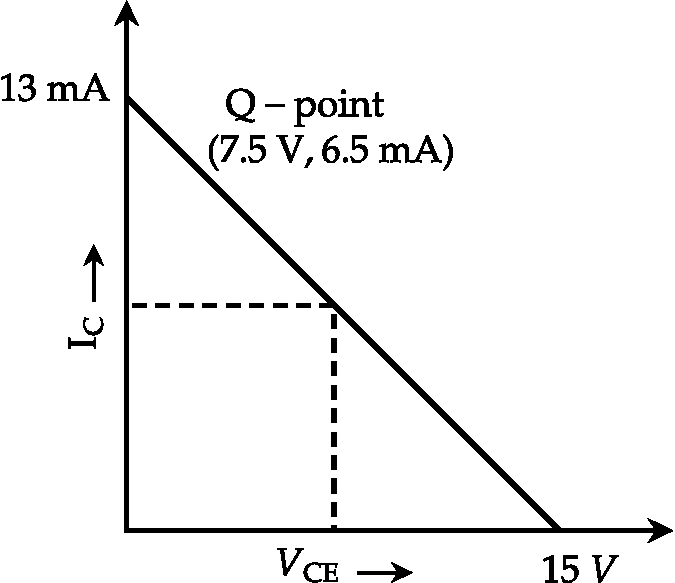
\includegraphics[height=4.5cm,width=5cm]{BJT-45}
\end{figure}
\end{tasks}
\begin{answer}
\begin{align*}
I_{B}&=\frac{V_{C C}-V_{B E}}{R_{B}+R_{E}}=\frac{15-0.7}{100 \times 10^{3}+100} \approx \frac{14.3}{100} m A\\
I_{C} \approx \beta I_{B} \approx 14.3 m A \approx 13 m A, V_{C E}&=V_{C C}-I_{C}\left(R_{C}+R_{E}\right)\\&=15-(900+100) \times 13 \times 10^{-3}=2 V\\
I_{C, S a t}&=\frac{\mathrm{V}_{\mathrm{CC}}}{\mathrm{R}_{\mathrm{C}}+R_{E}}=\frac{15}{1000}=15 \mathrm{~mA}
\end{align*}
So the correct answer is \textbf{Option (A)}
\end{answer}
	\item The current gain of the transistor in the following circuit is $\beta_{d c}=100$. The value of collector current $I_{C}$ is----------- $m A$
{	\exyear{GATE 2014}}
\begin{figure}[H]
\centering
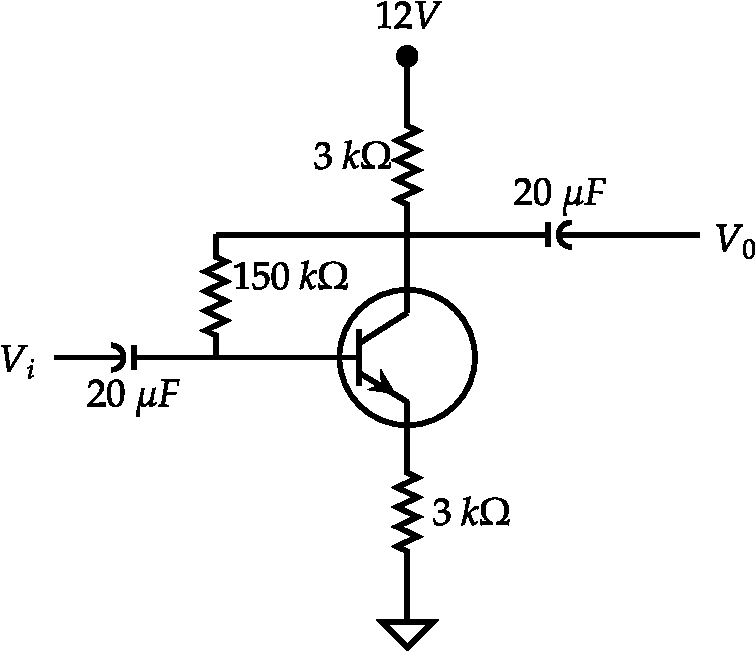
\includegraphics[height=7cm,width=8cm]{BJT-46}
\end{figure}
\begin{answer}
\begin{align*}
I_{B}&=\frac{V_{C C}-V_{B E}}{R_{B}+\beta\left(R_{C}+R_{E}\right)}=\frac{12-0}{150+100(3+3)}\\&=0.016 \mathrm{~mA} \Rightarrow I_{C}=\beta I_{B}=1.6 \mathrm{~mA}
\end{align*}
\end{answer}
	\item In the simple current source shown in the figure, $Q_{1}$ and $Q_{2}$ are identical transistors with current gain $\beta=100$ and $V_{B E}=0.7 \mathrm{~V}$\\
	\begin{figure}[H]
		\centering
		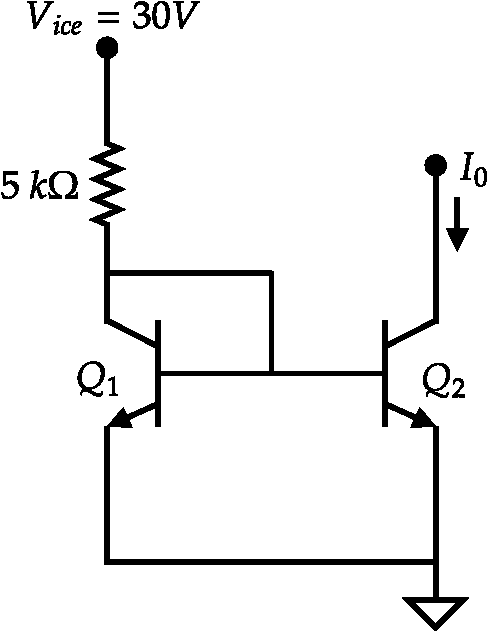
\includegraphics[height=6cm,width=5cm]{BJT-47}
	\end{figure}
	The current $I_{0}($ in $m A)$ is --------(upto two decimal places)
{	\exyear{GATE 2015}}
\begin{answer}
\begin{align*}
-V_{C C}+I_{C} R_{C}+V_{B E}&=0, I_{C}=\frac{30-0.7}{5}\\&=\frac{29.3}{5}=5.86 \mathrm{~mA}
\end{align*}
\end{answer}
	\item In the given circuit, the voltage across the source resistor is $1 V$. The drain voltage $($ in $V)$ is-----------
{	\exyear{GATE 2015}}
\begin{figure}[H]
\centering
\includegraphics[height=6.5cm,width=4.5cm]{BJT-48}
\end{figure}
\begin{answer}
\begin{align*}
V_{S}&=I_{D} R_{S} \Rightarrow I_{D}=\frac{1}{500} A \Rightarrow V_{D}\\&=V_{D D}-I_{D} R_{D}=25-\frac{1}{500} \times 5000 \Rightarrow V_{D}=15 V
\end{align*}
\end{answer}
	\item For the transistor shown in the figure, assume $V_{B E}=0.7 V$ and $\beta_{d c}=100$. If $V_{\text {in }}=5 V, V_{\text {out }}$ (in Volts) is ---------(Give your answer upto one decimal place)
{	\exyear{GATE 2016}}
\begin{figure}[H]
\centering
\includegraphics[height=7cm,width=5.5cm]{BJT-49}
\end{figure}
\begin{answer}
\begin{align*}
I_{B}=\frac{V_{i n}-V_{B E}}{R_{B}+\beta R_{E}}&=\frac{5-0.7}{200+100}\\&=\frac{4.3}{300} m A, I_{C}=\beta I_{B}=1.433 \mathrm{~mA}\\
V_{\text {out }}&=V_{C C}-I_{C} R_{C} \Rightarrow V_{\text {out }}\\&=10-1.433 \times 3=5.7 \mathrm{~V}
\end{align*}
\end{answer}
	\item For the transistor amplifier circuit shown below with $R_{1}=10 \mathrm{k} \Omega, R_{2}=10 \mathrm{k} \Omega, R_{3}=1 k \Omega$, and $\beta-99$. Neglecting the emitter diode resistance, the input impedance of the amplifier looking into the base for small ac signal is............. $k \Omega$. (up to two decimal places)
{	\exyear{GATE 2017}}
\begin{figure}[H]
\centering
\includegraphics[height=6cm,width=5cm]{BJT-50}
\end{figure}
\begin{answer}
\begin{align*}
Z_{i}&=Z_{b} \| R^{\prime}\text{ where }Z_{b} \approx \beta R_{3}=99 k \Omega\text{ and } R^{\prime}\\&=R_{1} \| R_{2}=5 k \Omega\\
\Rightarrow Z_{i}&=Z_{b} \| R^{\prime}=4.75 k \Omega
\end{align*}
\end{answer}
\item An $n$ - channel FET having Gate-Source switch-off voltage $V_{G S(\mathrm{OFF})}=-2 V$ is used to invert a $0-5 V$ square-wave signal as shown. The maximum allowed value of $R$ would be-------- $k \Omega$ (up to two decimal places).
{\exyear{GATE 2018}}
\begin{figure}[H]
\centering
\includegraphics[height=5.5cm,width=10cm]{BJT-51}
\end{figure}
\begin{answer}
0.70
\end{answer}
\end{enumerate}